\section{Auswertung}
\label{sec:Auswertung}

Zu Beginn der Messung wird die RF-Spule mit einer Frequenz von $f_{\text{HF}}=\qty{100}{\kilo\hertz}$ betrieben.
In \autoref{fig:oszilloskop} ist der Verlauf der Lichtintensität in Abhängigkeit der Magnetfeldstärke der Sweepspule
zu sehen.

\begin{figure} [H]
  \centering
  \includegraphics[height=8cm]{content/oszilloskop.jpg}
  \caption{Oszilloskopbild bei $f_{\text{HF}}=\qty{100}{\kilo\hertz}$.}
  \label{fig:oszilloskop}
\end{figure}

Auffällig sind hier die negativen Peaks der Lichtintensität, einmal bei $B=0$ und bei den beiden charakteristischen
Feldstärken der Rubidium Isotope $^{85}\symup{Rb}$ und $^{87}\symup{Rb}$.
Der Peak bei $B=0$ dient nur zu Kalibrierung und ist bei der weiteren Auswertung nicht von Interesse.

Das horizontale Magnetfeld setzt sich aus dem Feld der Sweepspule und dem Feld der anderen horizontalen Spule
zusammen. Die Felder der Spulen lassen sich direkt aus dem Strom berechnen, gemäß der Helmholtz-Gleichung:
\begin{equation}
  B =\mu_0 \frac{8NI}{\sqrt{125}R}
  \label{eq:Bfeld}
\end{equation}
Das Gesamtfeld ergibt sich aus der Summe der beiden Felder.
\begin{equation}
  B_{\text{ges}} = B_{\text{sweep}} + B_{\text{hor}}
  \notag
\end{equation}
Das Sweepfeld dient zur Variation des Magnetfeldes innerhlab eines festgelegten Bereichs, um die erwähnten Peaks auflösen zu können.
Das horizontale Feld erlaubt eine konstante Verschiebung dieses Bereiches, um die wandernden Peaks bei Erhöhung der HF-Frequenz
$f_{\text{HF}}$ im Oszilloskop verfolgen zu können.
Die Stromstärke der Sweepspule kann über die angelegte Spannung über einen Faktor von $0.1$ ermittelt werden, während die
Stromstärke der horizontalen Spule direkt gemessen wird. Die Messwerte sind im Anhang in \autoref{fig:messdaten} zu sehen.

\subsection{Bestimmung der g-Faktoren und der Kernspins}

Die HF-Frequenz $f_{\text{HF}}$ wird ausgehend von $\qty{100}{\kilo\hertz}$ in $\qty{100}{\kilo\hertz}$ Schritten erhöht,
bis eine Frequenz von $\qty{1}{\mega\hertz}$ erreicht ist.
Für jede Frequenz werden die Stromstärken der Spulen an den beiden Peaks am Oszilloskop abgelesen und anschließend wird
dann mithilfe von \eqref{eq:Bfeld} die den Peaks zugehörige Magnetfeldstärke berechnet.
Die Wertepaare für beide Isotope sind in \autoref{fig:plot} geplottet.

\begin{figure} [H]
  \centering
  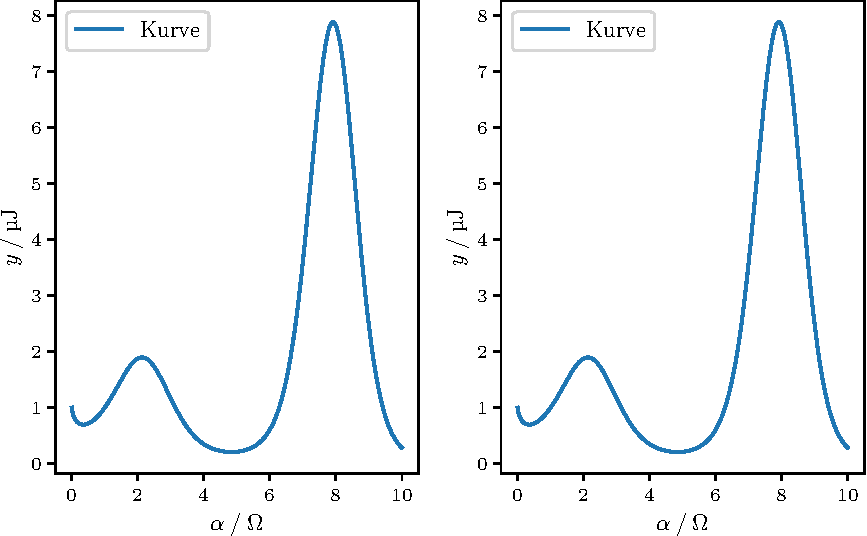
\includegraphics[height=8cm]{plot.pdf}
  \caption{Magnetfeldstärke $B$ an den Resonanzen in Abhängigkeit der RF-Frequenz $f_{\text{HF}}$, zusammen mit den zugehörigen Regressionsgraden.}
  \label{fig:plot}
\end{figure}

Gemäß \eqref{eq:Resonanz} lässt sich ein linearer Zusammenhang zwischen RF-Frequenz $f_{\text{HF}}$ und Magnetfeld $B$ herstellen:
\begin{equation}
  B = \frac{h}{g_F \mu_B}f
  \notag
\end{equation}
Ein linearer Fit der Form $B(f)=a*f+b$ wird durchgeführt, er ist in \autoref{fig:plot} eingezeichnet und liefert die Parameter:
\begin{align*}
  a_1 = \qty{1.431(0.007)e-10}{\tesla\per\hertz}, &&b_1 =\qty{2.54(0.04)e-05}{\tesla} \\
  a_2 = \qty{2.109(0.019)e-10}{\tesla\per\hertz}, &&b_2 =\qty{2.64(0.12)e-05}{\tesla}
\end{align*}
Die Parameter $b_1$ und $b_2$ beschreiben den horizontalen Versatz der Geraden, der durch die horizontale Komponente
des Erdmagnetfeldes verursacht wird. Daher kann aus ihrem Mitttelwert die Stärke des Erdmagnetfeldes berechnet werden: 
\begin{align*}
  B_{\text{Erde}} = \qty{25.9(0.6)}{\micro\tesla}
\end{align*}
Mithilfe der Fitparameter $a_1$ und $a_2$ kann nun durch umstellen der jeweilige g-Faktor $g_{\text{F}}$ der Isotope bestimmt werden.
\begin{align*}
  g_{\text{F}_1\text{,exp}} = \qty{0.4991(0.0024)}{} \\
  g_{\text{F}_2\text{,exp}} = \qty{0.3387(0.0031)}{}
\end{align*}
Die Ergebnisse liegen somit nah an den theoretischen Werten von $g_{\text{F}_1}=\frac{1}{2}$ und $g_{\text{F}_2}=\frac{1}{3}$.
Aus den g-Faktoren kann mithilfe von \eqref{eq:gf} der jeweilige Kernspin berechnet werden. Für die Berechnung von $g_J$ 
werden die Quantenzahlen $S=\frac{1}{2}$, $L=0$ und $J=L+S=\frac{1}{2}$ gemäß \cite{Optical_Pumping} verwendet.
Umstellen der Gleichung und einsetzen der Werte liefert die Kernspins:
\begin{align*}
  I_{1\text{,exp}} = \qty{1.504(0.010)}{} \\
  g_{2\text{,exp}} = \qty{2.452(0.027)}{}
\end{align*}
Die theoretischen Kernspins der beiden Isotope sind $I=2.5$ für $^{85}\symup{Rb}$ und $I=1.5$ für $^{87}\symup{Rb}$.
Somit handelt es sich beim Isotop 1 (1.Peak) um $^{87}\symup{Rb}$ und beim Isotop 2 (2.Peak) um $^{85}\symup{Rb}$.

\subsection{Isotopenverhältnis}

Um das Verhältnis der beiden Isotope zu bestimmen, werden die Höhen der Absorptionspeaks miteinander verglichen.
Dafür wird das Oszilloskopbild aus \autoref{fig:oszilloskop} verwendet, die RF-Frequenz $f_{\text{HF}}$ beträgt
hier also $\qty{100}{\kilo\hertz}$.
Die Höhen der Peaks in Pixeln Betragen $1780$ für den ersten Peak und $748$ für den zweiten.
Somit berechnet sich das Verhältnis zu:
\begin{align*}
  \frac{^{85}\symup{Rb}}{^{87}\symup{Rb}} \approx \qty{0.42}{}
\end{align*}
Dies ist etwas höher als das natürliche Verhältnis von $0.38$. Der Grund dafür besteht darin, dass zugunsten einer
besseren Messbarkeit das $^{85}\symup{Rb}$ angereichert wurde, um einen größeren Peak zu erhalten.